\documentclass{tccv_full}
\usepackage[english]{babel}
\usepackage{epsfig}
\usepackage{wrapfig}
% im_convert.exe "C:\Users\Ricardo\Google Drive\Documentos\CV\FullSizeRender.png" eps3:"C:\Users\Ricardo\Google Drive\Documentos\CV\FullSizeRender.eps"

\begin{document}

\part{Bruno Justino Garcia Praciano}
\personal[www.lasp.unb.br]
{Bras\'ilia-DF, Brazil}
{+55 (61) 98355-0909}
{bjpraciano@gmail.com}
{\mbox{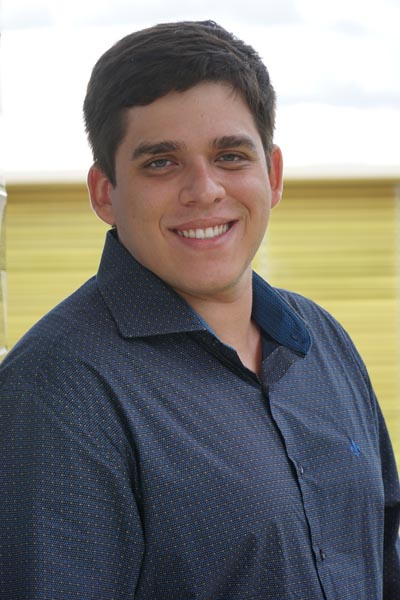
\includegraphics[width=0.14\textwidth, trim=0 0cm 0 0]{CV1}}}

\vspace{1.9cm}

\section{Summary}

In this r\'esum\'e you can find that my expertise is focused on machine learning techniques specially in text mining. I also have a deep interest in other types of machine learning applications. I have been recently working on face recognition and peer to peer networks in my actual position. My background also includes full stack development and biomedical engineering product development.

\vspace{-0.4cm}
\section{Professional Experience}

		{\large April 2019 -- Present:	\textbf{Legal Labs Artificial Intelligence}}
	Activities:
	\begin{itemize}
		\item{Intelligence platform mass process based on prediction}

		{\small
			\subitem - TensorFlow
			\subitem - Pytorch
			\subitem - Spark
			\subitem - Python
			\subitem - Natural Language Processing
			\subitem - WebCrawler
		} 
	\end{itemize}
	{\large October 2017 -- Present:	\textbf{Universal Internet of Things Laboratory}}
	Activities:
	\begin{itemize}
		\item \textsf{Implementation of face recognition using IoT}
		{\small
			\subitem - Face Recognition
			\subitem - Deep Learning
			\subitem - OpenCV
			\subitem - Python
			\subitem - RaspberryPI
		} 
		\item \textsf{Peer to Peer Network to IoT devices}
		{\small
			\subitem - Sockets
			\subitem - Chord Network
		}	

	\end{itemize}

	\vspace{0.7cm}
	{\large September 2017 -- August 2018:
	\textbf{Robotic Process Automation Developer at DOZE}\\}
	Activities:
	\begin{itemize}
		\item \textsf{Robotic Process Automation}
			{\small 
			\subitem - WDG Automation 
			\subitem - Automation Anywhere
			\subitem - Scrapy and Selenium
			}
		
		\item \textsf{Customer Service}
			{\small 
			\subitem - Marketing
			\subitem - Direct Contact with clients
			}
		
	\end{itemize}
	
	\vspace{0.7cm}
	{\large June. 2016 -- September 2017: \textbf{CTO at Eduqc.com}\\}
	\begin{itemize}
		\item \textsf{Team Management with Agile with Scrum}
		\item \textsf{Full Stack development}
		{\small 
		\subitem - Laravel, Python, Javascript, Vue
		\subitem - SQL, AWS }
	\end{itemize}
	
	{\large Jan. 2015 -- April. 2017: \textbf{Researcher at Biomedical Engineering Laboratory - UnB.} \\	
	
	
\section{Education}

	{March 2019 -- Present}: \textbf{Master of Science in Electronics and Automation Engineering}\\
	{University of Bras\'ilia (UnB)}\\	
	
	
	\vspace{0.5cm}
	


	{April 2013 -- December 2018}: \textbf{Computer Engineer Bachelor Degree}\\
	{University of Bras\'ilia (UnB)}\\
	
	


\section{Communication skills}

\begin{factlist}
\item{Portuguese}{Native speaker}
\item{English}{Oral and written: advanced}
\item{German}{Oral and written: basic}
\item{Spanish}{Oral and written: basic with good understandability due to similarity}
\end{factlist}

\section{Software skills}

\begin{factlist}

\item{Good level}
     {Python, R, Sci-kit Learn, TensorFlow, NLP, Javascript, Vue, C, Matlab, PHP, HTML, CSS, \LaTeX, Linux, Docker, SQL}

\item{Intermediate}
     { React, Node, Django, MongoDB}



\end{factlist}
\section{Research Interests}
Artificial Intelligence, Internet of Things, Data Mining

\section{Selected Volunteer Activities}
President and founder of the first IEEE Vehicular Technology Society (VTS) chapter in Brazil.\\
Founder and Publication Chair of the Workshop on Communication Networks and Power Systems (WCNPS) in 2017 and 2018.



\section{Selected Publications}

	$[1]$ \textbf{B. Praciano}, J. P. C. L. da Costa, J. P. A. Maranh\~ao, J. B. Prettz, R. T. de Sousa Jr. and F. Mendonca, “Spatio-Temporal Trend Analysis of the Brazilian Elections based on Twitter Data, ” 2018 IEEE International Conference on Data Mining Workshop (ICDMW), Singapore, \\
\end{document}
